%!TEX root = ../main.tex

\begin{titlepage}

    
\includegraphics[height=2.5cm]{images/cover/logo-dhbw.pdf}
    \IfStrEq{\showCompanyLogo}{true}{
        \hfill
        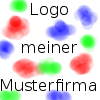
\includegraphics[height=2.5cm]{images/cover/logo-company.png}
    }
    
    \begin{center}
        \vspace*{14mm}
        \begin{spacing}{1.4}
            {\LARGE\textbf\documentTitle}
        \end{spacing}
        \vspace*{13mm}
        {\large\textbf\documentTypePhrase}\\

        % degre only for bachelor thesis
        \ifDocType{T3300}{
            \vspace*{13mm}
            \degreePhrase\\[2mm]
            {\textbf\degree}\\
        }

        \IfStrEq{\showLecture}{true}{
            \vspace*{13mm}
            \lecturePhrase\\[2mm]
            {\textbf\lecture}\\
        }

        \vspace*{13mm}
        \departmentPhrase\space\department\\[1mm]
        \locationUniversityPhrase{} \locationUniversity\\

        \vspace*{8mm}
        \documentAuthorPhrase\\[8mm]
        {\renewcommand{\arraystretch}{1.45}%
        \begin{tabular}{@{}l@{\hspace{12mm}}l@{}}
            \textbf{Name} & \textbf{\matriculationNumberPhrase} \\[1mm]
            \autorEins & \matrikelEins \\
            \autorZwei & \matrikelZwei \\
            \autorDrei & \matrikelDrei \\
            \autorVier & \matrikelVier \\
        \end{tabular}}\\

        \vspace*{16mm}
        \releaseDate
    \end{center}

    \vfill
    {\renewcommand{\arraystretch}{1.3}%
    \begin{tabular}{@{}l@{\hspace{10mm}}l@{}}
        \textbf{\coursePhrase}    & \course    \\
        \textbf{\evaluatorPhrase} & \evaluator
    \end{tabular}}
\end{titlepage}
